% Skeleton report for Assignment S1:Percolation, in Reiknirit, fall 2020, at Reykjavik University
%  (c) 2017, Magnus M. Halldorsson
%
% Builds on the assignment Percolation at Princeton University, (c) Kevin Wayne
%
% Format is based on the following document:
% A basic LaTeX document for a handin with a standard RU title page
%  (c) 2013, Tómas Ken Magnússon, 

% If you want the title to appear on a separate page, change notitlepage to titlepage
\documentclass[11pt,a4paper,notitlepage]{article}
\usepackage[utf8]{inputenc}
\usepackage[T1]{fontenc}
% If your hand-in is in icelandic change english to icelandic
% Note: This has nothing to do with Icelandic characters, they
% can always be used. This just tells other packages what
% language you are using and changes the hyphenation used by LaTeX
% If icelandic is selected2 a shorthand, "` and "', is also included
% for Icelandic quotation marks. They can also obtained by using
% ,, and ``
\usepackage[english]{babel}
\usepackage{amsmath, amsthm, amssymb, amsfonts}
\usepackage{graphicx}
\usepackage{enumerate}
% To use the whole A4-page
% See: ftp://ftp.tex.ac.uk/tex-archive/macros/latex/contrib/geometry/geometry.pdf
% and http://en.wikibooks.org/wiki/LaTeX/Document_Structure
\usepackage{geometry}
% For header and footer
% See: ftp://ctan.tug.org/tex-archive/macros/latex/contrib/ fancyhdr/fancyhdr.pdf
% and http://en.wikibooks.org/wiki/LaTeX/Document_Structure
\usepackage{fancyhdr}
% For prettier tables
% See: http://ctan.mackichan.com/macros/latex/contrib/booktabs/booktabs.pdf
% and  http://en.wikibooks.org/wiki/LaTeX/Tables
%\usepackage{booktabs}
\usepackage{listings} % For code listing

% \usepackage{sagetex}
\usepackage{hyperref}
\usepackage{caption}
\usepackage[usenames,dvipsnames,svgnames,table]{xcolor}
\usepackage{subfig}  % To fit two tables side-by-side

\usepackage{pgfplots} % To create the plots that we are going to need

%%%%%%%%%%%%%%%%%%%%%%%%%%%%%%%%%%%%%%%%%%%%%%%%%%%%%%%%%%%%%
%                        Setup
%%%%%%%%%%%%%%%%%%%%%%%%%%%%%%%%%%%%%%%%%%%%%%%%%%%%%%%%%%%%%

% Set the margins of the paper. By default LaTeX uses huge margins
\geometry{includeheadfoot, margin=2.5cm}
% you can also use
% \geometry{a4paper}
% End of margins setup

% Settings for listings
\lstset{language=Java,numbers=left,backgroundcolor=\color{light-gray},
        basicstyle=\scriptsize\ttfamily,frame=single,tabsize=4,
        captionpos=t, numbers=left,
        keywordstyle=\color{javapurple}\bfseries,
        stringstyle=\color{javared},
        commentstyle=\color{javagreen},
        morecomment=[s][\color{javadocblue}]{/**}{*/},}
% End of settings for listings

% Custom colors for listings
\definecolor{light-gray}{gray}{0.95}
\definecolor{javared}{rgb}{0.6,0,0} % for strings
\definecolor{javagreen}{rgb}{0.25,0.5,0.35} % comments
\definecolor{javapurple}{rgb}{0.5,0,0.35} % keywords
\definecolor{javadocblue}{rgb}{0.25,0.35,0.75} % javadoc
% End of custom colors for listings


% Fill in any relevant information
% Leave the fields inside the {} empty if they do not apply
\newcommand{\semester}{Fall 2020}
\newcommand{\coursename}{Reiknirit}
\newcommand{\courseid}{T-301-REIR}
\newcommand{\assignment}{S1: Percolation}
\newcommand{\problemtitle}{Problem}
\newcommand{\dateofcompilation}{\today}

%% Information about you --- FILL THIS OUT
\newcommand{\group}{???}                   %%%  CHANGE THIS """
\newcommand{\teachingassistant}{TA's: All of them}   %%%  CHANGE THIS """
%\newcommand{\ssn}{kt. 123456-7890}             
%\newcommand{\students}{    Name of Student                             }
%\newcommand{\studentemail}{
% myEmails@ru.is                            
%}
 
% Setup header and footer
% Headers
\pagestyle{fancy} % To get the header and footer
\chead{\small \textsc{\assignment}}
\rhead{\small \textsc{\coursename}}
\lhead{\small \textsc{StudyGroup \group}}
% Footers
%\lfoot{Left footer text}
%\cfoot{\thepage} % This is the default behaviour
%\rfoot{Right footer text}


% Custom dot for itemize
\renewcommand{\labelitemi}{$\cdot$}

% If you don't want a line below the header or above the footer,
% change the appropriate header/footerrulewidth to 0pt
\setlength{\headheight}{15.2pt} % This is set to avoid a warning
\renewcommand{\headrulewidth}{0.4pt}
\renewcommand{\footrulewidth}{0.4pt}
% End of header and footer setup

% Setup Problem/Solution environments // You probably don't need this
%\theoremstyle{plain}
%\newtheorem{problem}{Dæmi}
%\theoremstyle{remark}
%\newtheorem*{solution}{Lausn}
% End of Problem/Solution environments setup
%\theoremstyle{plain}
%\newtheorem*{proposition}{Proposition}

\DeclareCaptionLabelFormat{andtable}{#1~#2  \&  \tablename~\thetable}

% The title page
\newcommand{\maketitlepage}[1]
{
    \begin{titlepage}

        \begin{center}
            \includegraphics[width=0.55\textwidth]{./rulogo.png}\\[1.5cm]

            \textsc{\huge \semester}\\[0.8cm]

            {\textsc{\Huge \courseid, \coursename}}\\[0.4cm]
            \textsc{\LARGE }\\[2.5cm]

            \textbf{\textsc{\Huge #1}}\\[2.5cm]


            \textsc{\LARGE (Ketamine addict), (illugif@ru.is)}\\  %%%  CHANGE THIS """
            \textsc{\LARGE (Apple fanboy), (peturs19@ru.is)}\\[0.6cm]  %%%  CHANGE THIS """

            \textsc{\LARGE Study Group: \group}\\[1cm] 
            \textsc{\Large \dateofcompilation}


        \end{center}

        \vfill

        % You may also want to add the name of your teaching assistant
        \begin{flushleft}
            \textsc{\Large \teachingassistant}
        \end{flushleft}

    \end{titlepage}
}
\newcommand{\command}[1]{\texttt{\textbackslash{}#1}}

\newcommand{\explanation}[1]{}  %% Use this when turning in the report
% \newcommand{\explanation}[1]{\begin{quote}\emph{#1} \end{quote}}  %% Use this to include directions

%%%%%%%%%%%%%%%%%%%%%%%% END OF SETUP %%%%%%%%%%%%%%%%%%%%%%%%


\begin{document}
% Create the title page
    \maketitlepage{\assignment}

\explanation{Directions on performing the assignment are showed here in italics (like this). These should not be included in the report you submit.}

 \section{Introduction}
\explanation{State the objective(s) of the exercise. Ask yourself: Why did I perform the
  experiment? What did I aim to achieve? Provide background about the subject
  matter, as needed (what are union-find data structures good for?). Include
  the purpose of the different steps.
}
    The objective of the exercise is to find out if a N-by-N grid perculates, or better said, find the "magic" ratio between open and closed sites that makes the system perculate.
    We preformed the exercise to give us a better understanding of the problem at hand and understand how to utilize the different union-like structures.
    Our aim was to code the problem with different union like structures and then test it vigorously by using our Stats class.

    Percolation\\

    Perculation (Útskýra hvað í fokkanum perculation er - copya frá lýsingu ?)

  \subsection{Setup and Methods}
\explanation{ Describe how you performed the exercise. Write about what you actually did
  rather than what you were supposed to do. Be concise;  only give the
  necessary details a person in the same field needs to perform the exercise.
  Write in narrative form (i.e., telling a story) rather than a numbered list
  format. Describe both the set-up (hardware, OS, software, tools) and the testing
  process. Refer to the classes written.}
    We did the project on "macc details" using IntelliJ from jetbrains for java development and we used java11. We started on figuring out how we want to store all of the data and how we can do that efficiently!
    We started with a integer grid so we could get the row and col and get the value but a matrix if integers takes alot of memeory, so we settled on using a boolean matrix to keep track whether the site is open or not,
    but that created a problem, how are we going to find the index for the union data structure? Simple! We devised a plan! Since we know that it's a N-by-N grid then we can calculate the index for the data structure,
    the formula is as such:
    \begin{equation}
        index = (row * N) + col 
    \end{equation}
    After we found that out we started programming, we then figured out that we need to find an efficient way to store pairs of row number and column number, we created a private Pair class within the Perculation class,
    The pair class is as simple as it gets, it stores the row number and the column number.\\

    When we finished that we went about of writing the open function, the open function simply opens the site and then checks if any other neighbouring cells are open, if so we connect them to the union data structure. But how are we going to find the neighbours ?
    By writing methods! Private methods to be exact, We wrote a method that gets the neighbouring cells row number and column number and then we wrote another private method that checks if the row numbers and column numbers are valid within the N-by-N matrix the system is in. 
    
    Private methods 






\subsection{Implementation}
% /******************************************************************************
\explanation{Describe how you implemented the \texttt{Percolation} datatype. How did you check
whether the system percolates?}

%  *****************************************************************************/

\explanation{Describe how you implemented \texttt{PercolationStats}.}

\section{Results}
\explanation{Describe the experimental results in words, referring to the tables.}

\paragraph{Percolation constant}
\explanation{What estimate of the percolation constant did your experiments suggest?}

\subsection{Quick-Find}

\explanation{Using Percolation with \texttt{QuickFindUF.java}, fill in the table below such that the $N$ values are
  multiples of each other.  Also fill in the second table, using a fixed, relevant value of $N$.}

\paragraph{Results}

\begin{table}[htbp]
%  \small
  \centering
  \caption{Using Java11 LTS}
  \subfloat[QuickFind results]{   %% CHANGE THE CAPTIONS
        \label{tab:table1}
        \begin{tabular}{|r|r| c | c | c | c |}
        \hline
        $N$ & $T$ & Total Running Time(s) & Confid.(low) & Avg Threshold & Confid.(high)\\ 
        \hline
        200 & 100 & 20.886 & 0.5916614856943488 & 0.593601000905037 & 0.5955405161157251 \\
        200 & 200 & 58.478 & 0.5915249435319724 & 0.5928471261262893 & 0.5941693087206062 \\
        400 & 100 & 301.269 & 0.5922470075078308 & 0.5933678120374679 & 0.594488616567105 \\
        400 & 200 & 899.393 & 0.5915991882347434 & 0.5923998117446899 & 0.5932004352546364 \\
        \hline
        \end{tabular}
  }

\end{table}

\begin{figure}[!ht]
    \label{fig:plot2}
      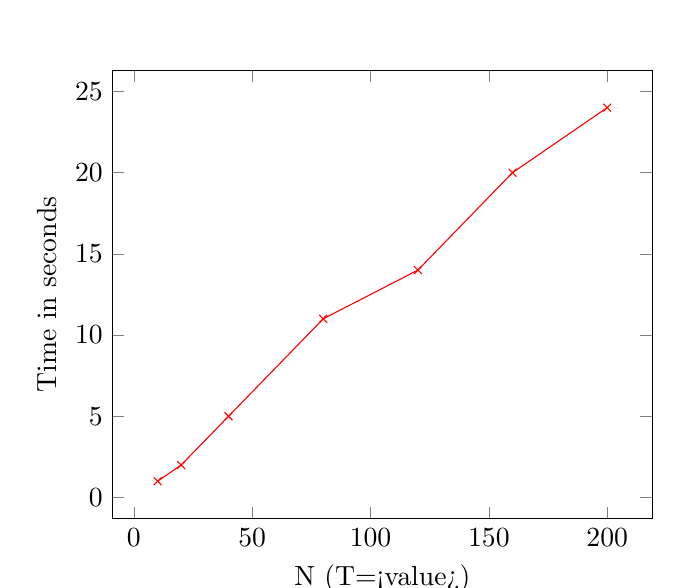
\begin{tikzpicture} 
        \begin{axis}[ xlabel=N (T{=}<value>), ylabel=Time in seconds] 
          \addplot[color=red,mark=x] coordinates {
            (10,1) 
            (20,2) 
            (40,5) 
            (80,11) 
            (120,14) 
            (160,20) 
            (200,24)
        };
        \end{axis} 
      \end{tikzpicture}
    \caption{This is the caption for the plot}
    \end{figure}


\explanation{Refer to these table in the text! Give the time results
  also in a plot, possibly in a log-log scale. For bonus points,
  also compute confidence intervals for the time and add them to your
  plot.}


% Example plot
    \begin{figure}[!ht]
        \label{fig:plot1}
        \centering
        A chart should be included here.
%        \includegraphics[width=0.6\textwidth]{chart.pdf}
        \caption{This is the caption for the chart.}
    \end{figure}


\paragraph{Time complexity}
\explanation{
Give a formula (using tilde notation) for the running time (in seconds) of 
\texttt{PercolationStats.java} as a function of both $N$ and $T$. Be sure to give both 
the coefficient and exponent of the leading term. Your coefficients should 
be based on empirical data and rounded to two significant digits, such as 
$5.3 \cdot 10^{-8} \cdot N^{5.0} T^{1.5}$.}

Running time as a function of $N$ and $T$:  $\sim$ 

\explanation{Explain how you come up this running time}
% \textbf{Reasoning:}

\subsection{Weighted Quick-Union}
\begin{table}[htbp]
    %  \small
    \centering
    \caption{Using Java11 LTS}
    \subfloat[Weighted QuickUnion results]{   %% CHANGE THE CAPTIONS
    \label{tab:table2}
    \begin{tabular}{|r|r| c | c | c | c |}
    \hline
        $N$ & $T$ & Total Running Time(s) & Confid.(low) & Avg Threshold & Confid.(high)\\ 
    \hline
        200 & 100 & 0.373 & 0.5895962947979569 & 0.591609999537468 & 0.593623704276979 \\
        200 & 200 & 0.659 & 0.5912201780959143 & 0.5912201780959143 & 0.594014821560763 \\
        400 & 100 & 1.415 & 0.5906189738214016 & 0.5918477481603622 & 0.5930765224993229 \\
        400 & 200 & 2.302 & 0.592641312851526 & 0.5934378761053085 & 0.594234439359091 \\
    \hline
    \end{tabular}
}    
\end{table}
% /******************************************************************************
\explanation{Repeat the previous subsection, but using WeightedQuickUnionUF.java.}
%  *****************************************************************************/
% /*** Include all of the previous subsection here ***/

\subsection{Memory Usage}
% /**********************************************************************
\explanation{
How much memory (in bytes) does a \texttt{Percolation} object use to store
an $N$-by-$N$ grid? Use the 64-bit memory cost model from Section 1.4
of the textbook and use tilde notation to simplify your answer.
Briefly justify your answers.}

\explanation{Include the memory for all referenced objects (deep memory).}
%  **********************************************************************/


\subsection{Discussion/Conclusions}

\explanation{Summarize briefly the outcomes. 
What do they mean? How successful was the experiment? 
Qualify your statements.}

\section{About This Solution}

Have you taken (part of) this course before:

Hours to complete assignment (optional):


% /******************************************************************************
%  *  After reading the course rules on collaboration policy, answer the
%  *  following short quiz. This counts for a portion of your grade.
%  *  Write down the answers in the space below.
%  *****************************************************************************/
\subsection{Quiz on Collaboration}

\begin{enumerate}
\item How much help can you give a fellow student taking REIR?
\begin{enumerate}
\item None. Only the TAs can help.
\item You can discuss ideas and concepts but students can get help
    debugging their code only from a TA, or
    student who has already passed REIR.
\item You can help a student by discussing ideas, selecting data
    structures, and debugging their code.
\item You can help a student by emailing him/her your code.
\end{enumerate}

\textbf{Answer:} 

%\begin{enumerate}
\item What is the expectation when partnering?
\begin{enumerate}
 \item You and your partner split the assignment between you and solve the parts separately.
 \item You and your partner discuss all the problems together, but code separately.
 \item You and your partner discuss the problems and write all the code together.
\end{enumerate}
\end{enumerate}

\textbf{Answer:} 
 
\subsection{Known Bugs / Limitations.}
% /******************************************************************************
%  *  Known bugs / limitations.
%  *****************************************************************************/

\subsection{Help Received}
% /******************************************************************************
\explanation{
Describe whatever help (if any) that you received.
Don't include readings, lectures, and classes, but do
include any help from people (including course staff, lab TAs,
classmates, and friends) and attribute them by name.}
%  *****************************************************************************/


\subsection{Problem Encountered}
% /******************************************************************************
\explanation{
Describe any serious problems you encountered.                    }
%  *****************************************************************************/



\subsection{Comments}
% /******************************************************************************
\explanation{
List any other comments here. Feel free to provide any feedback   
on how much you learned from doing the assignment, and whether    
you enjoyed doing it.}
% *****************************************************************************/




\end{document}

%%%% Optional material


    \pagebreak
    \section*{Appendix I: Source code listings}
    Optional.

    \subsection*{Acknowledgement}

    % Environment for listing code
    \begin{lstlisting}[caption={This is a caption.},label={lst:array1}]
public class This is a class {

    // This is a comment
    public static double thisIsAFunction(int N) {
        QuickUnionUF uf = new QuickUnionUF(N);
        return something;
    }
    public static void main(String[] args) { 
        int T = 50;
    }
} 
    \end{lstlisting}

% Example reference:    See Listing \hyperref[lst:array1]{1}.


    \pagebreak
    \section*{Appendix II}
    Optional.

    \listoftables
    \listoffigures
    \lstlistoflistings
    \bibliographystyle{plain}
    \bibliography{s1.bib}

\end{document}


